Para mejorar una red neuronal, el objetivo es encontrar pesos y sesgos que minimicen la función de coste. Como las redes neuronales suelen tener un gran número de pesos y sesgos, suele tratarse de un problema de optimización de gran dimensión.

El descenso de gradiente es un algoritmo de optimización iterativo que se utiliza para encontrar los valores de los parámetros (pesos y sesgos) que minimizan una función de coste. El algoritmo funciona calculando el gradiente de la función de coste con respecto a los parámetros con el objetivo de minimizar su salida, esto se muestra en la Figura \ref{fig:Gradiente}. Luego se actualizan los parámetros en la dirección opuesta al gradiente, lo que conduce a una disminución de la función de coste. Este proceso se repite hasta que se alcanza un mínimo local o global de la función de coste, lo que indica que se han encontrado los mejores parámetros para el modelo.

\begin{figure}[H]
    \begin{center}
    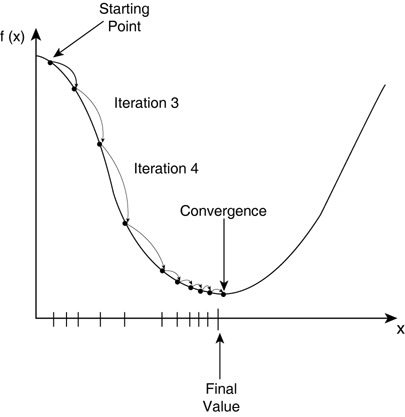
\includegraphics[width=0.7\textwidth]{commons/Fig7.jpg}
    \caption{Ilustración del proceso de descenso de gradiente.}
    \label{fig:Gradiente}
    \cite{rafii18}
    \end{center}
\end{figure}
